%%%%%%%%%%%%%%%%%%%%%%%%%%%%%%% main.tex %%%%%%%%%%%%%%%%%%%%%%%%%%%%%%%
%                                                                      %
% --------------------- Report Template IST [EN] --------------------- %
%                                                                      %
%       João Marafuz Gaspar                                            %
%       Departamento de Engenharia Eletrotécnica e de Computadores     %
%       Instituto Superior Tecnico                                     %
%       Av. Rovisco Pais                                               %
%       1049-001 Lisboa                                                %
%       Portugal                                                       %
%       E-mail: joao.marafuz.gaspar@tecnico.ulisboa.pt                 %
%                                                                      %
%  Created:       Jul 30, 2022                                         %
%  Last Modified: May 18, 2024                                         %
%                                                                      %
%%%%%%%%%%%%%%%%%%%%%%%%%%%%%%%%%%%%%%%%%%%%%%%%%%%%%%%%%%%%%%%%%%%%%%%%
%  Revision history                                                    %
%  v1 - 2022/07/30 - original template                                 %
%  v2 - 2023/04/06 - change superscript in the cover, updated font,    %
%                    added subfigures and table                        %
%  v3 - 18/05/2024 - update for using only one font, known by the name %
%                    of CMU Serif Roman                                %
%%%%%%%%%%%%%%%%%%%%%%%%%%%%%%%%%%%%%%%%%%%%%%%%%%%%%%%%%%%%%%%%%%%%%%%%
%                              Preamble                                %
%%%%%%%%%%%%%%%%%%%%%%%%%%%%%%%%%%%%%%%%%%%%%%%%%%%%%%%%%%%%%%%%%%%%%%%%

% ----------------------------------------------------------------------
% Set the document class
% ----------------------------------------------------------------------
\documentclass[12pt]{article}

% ----------------------------------------------------------------------
% Define external packages, language, margins, fonts, new commands 
% and colors
% ----------------------------------------------------------------------
\usepackage[utf8]{inputenc} % Codification
\usepackage[english]{babel} % Writing idiom

\usepackage[export]{adjustbox} % Align images
\usepackage{amsmath} % Extra commands for math mode
\usepackage{amssymb} % Mathematical symbols
\usepackage{anysize} % Personalize margins
    \marginsize{2cm}{2cm}{2cm}{2cm} % {left}{right}{above}{below}
\usepackage{appendix} % Appendices
\usepackage{cancel} % Expression cancellation
\usepackage{caption} % Captions
    \captionsetup{labelfont={bf}}
\usepackage{cite} % Citations, like [1 - 3]
\usepackage{color} % Text coloring
\usepackage{fancyhdr} % Head note and footnote
    \pagestyle{fancy}
    \fancyhf{}
    \fancyhead[L]{\footnotesize CSE-302} % Left of Head note
    \fancyhead[R]{\footnotesize Hacker's Lair} % Right of Head note
    \fancyfoot[L]{\footnotesize CSE} % Left of Footnote
    \fancyfoot[C]{\thepage} % Center of Footnote
    \fancyfoot[R]{\footnotesize MIST} % Right of Footnote
    \renewcommand{\footrulewidth}{0.4pt} % Footnote rule
\usepackage{float} % Utilization of [H] in figures
\usepackage{graphicx} % Figures in LaTeX
\usepackage[colorlinks = true, plainpages = true, linkcolor = istblue, urlcolor = istblue, citecolor = istblue, anchorcolor = istblue]{hyperref}
\usepackage{indentfirst} % First paragraph
\usepackage[super]{nth} % Superscripts
\usepackage{siunitx} % SI units
\usepackage{subcaption} % Subfigures
\usepackage{titlesec} % Font
    \titleformat{\section}{\Large\bfseries}{\thesection}{1em}{}
    \titleformat{\subsection}{\large\bfseries}{\thesubsection}{1em}{}
    \titleformat{\subsubsection}{\normalsize\bfseries}{\thesubsubsection}{1em}{}
    \fancyfoot[C]{\thepage}

% Random text (not needed)
\usepackage{lipsum}
\usepackage{duckuments}

% New and re-newcommands
\newcommand{\sen}{\operatorname{\sen}} % Sine function definition
\newcommand{\HRule}{\rule{\linewidth}{0.5mm}} % Specific rule definition
\renewcommand{\appendixpagename}{\LARGE Appendices}

% Colors
\definecolor{istblue}{RGB}{3, 171, 230}
\definecolor{dkgreen}{rgb}{0,0.6,0}
\definecolor{gray}{rgb}{0.5,0.5,0.5}

%%%%%%%%%%%%%%%%%%%%%%%%%%%%%%%%%%%%%%%%%%%%%%%%%%%%%%%%%%%%%%%%%%%%%%%%
%                                 Document                             %
%%%%%%%%%%%%%%%%%%%%%%%%%%%%%%%%%%%%%%%%%%%%%%%%%%%%%%%%%%%%%%%%%%%%%%%%
\begin{document}

% ----------------------------------------------------------------------
% Cover
% ----------------------------------------------------------------------
\begin{center}
    \begin{figure}
        \centering
        
\includegraphics[width=0.75\linewidth]{logo.png}
        \label{fig:enter-label}
    \end{figure}
    \mbox{}\\[2.0cm]
    \textsc{\Huge Database Management Systems Sessional}\\[2.5cm]
    \textsc{\Large Subject code: CSE-302}\\[2.0cm]
    \textsc{\LARGE Project Proposal}\\[2.0cm]
    \HRule\\[0.4cm]
    {\Large \bf {Title -- Hacker's Lair}}\\[0.2cm]
    \HRule\\[1.5cm]
\end{center}

\begin{flushleft}
    \textbf{\large Group members:}
\end{flushleft}

\begin{center}
    \begin{minipage}{0.5\textwidth}
        \begin{flushleft}
            \large Iftekharul Islam\\
            \large Mohammad Sadman Shafiq\\
            \large Tasnuva Islam\\
            \large Sadia Jahan Moon\\
        \end{flushleft}
    \end{minipage}%
    \begin{minipage}{0.5\textwidth}
        \begin{flushright}
            {\texttt{\large 202214024\\}}
            {\texttt{\large 202114065\\}}
            {\texttt{\large 202114103\\}}
            {\texttt{\large 202114085\\}}
        \end{flushright}
    \end{minipage}
\end{center}
\begin{flushleft}
    \large $\boxed{\text{\bf Group } 4}$\\[4.0cm]
\end{flushleft}
    
% \begin{center}
%     \large \bf 2023/2024 -- \nth{2} Semester, P4
% \end{center}

\thispagestyle{empty}

% \setcounter{page}{0}

\newpage
% \begin{center}
%     \large \bf 2023/2024 -- \nth{2} Semester, P4
% \end{center}


% ----------------------------------------------------------------------
% Contents
% ----------------------------------------------------------------------
\tableofcontents 

\newpage

% ----------------------------------------------------------------------
% Body
% ----------------------------------------------------------------------

\sectionfont{\setcounter{secnumdepth}{2}}
\begin{document}

\section{Description}
Hacker's Lair is a platform designed to ensure CTF enthusiasts practice their skills on a daily and weekly basis. It is a platform that allows contests to be hosted at both the local and official levels. Our goal is to develop a website framework for organizing CTF contests. This platform organizes cyber security learning materials and resources, providing a clear roadmap for CTF enthusiasts, free of cost. It'll also be easy to navigate.


\section{Objectives}
\begin{itemize}
    \item To provide a platform for cyber security enthusiasts to test their skills.
    \item To develop a system for organizing CTF (capture-the-flag) contests.
    \item To gather all the learning materials and roadmap related to cyber security.
\end{itemize}
\section{Interviews and Surveys}
\subsection{Visiting organization: MIST Cybersecurity Club (MCSC)\\} 
MIST Cybersecurity Club provides advanced cybersecurity training in the Cyber-range (only cyber-range in Bangladesh), digital intelligence lab and online. The lessons are about different categories of cybersecurity/CTF problems, vulnerabilities found in websites/apps. They worked with governmental organizations like BGD e-GOV CIRT (Bangladesh Government’s e-Government Computer Incident Response Team) and also multiple national and international organizations like RICSEC, HackTheBox, PhoenixCTFs etc. They also host regular CTFs in collaboration with RICSEC. We spoke with Easin Arafat, the president of MCSC.\\
\begin{figure}[h]
    \centering
    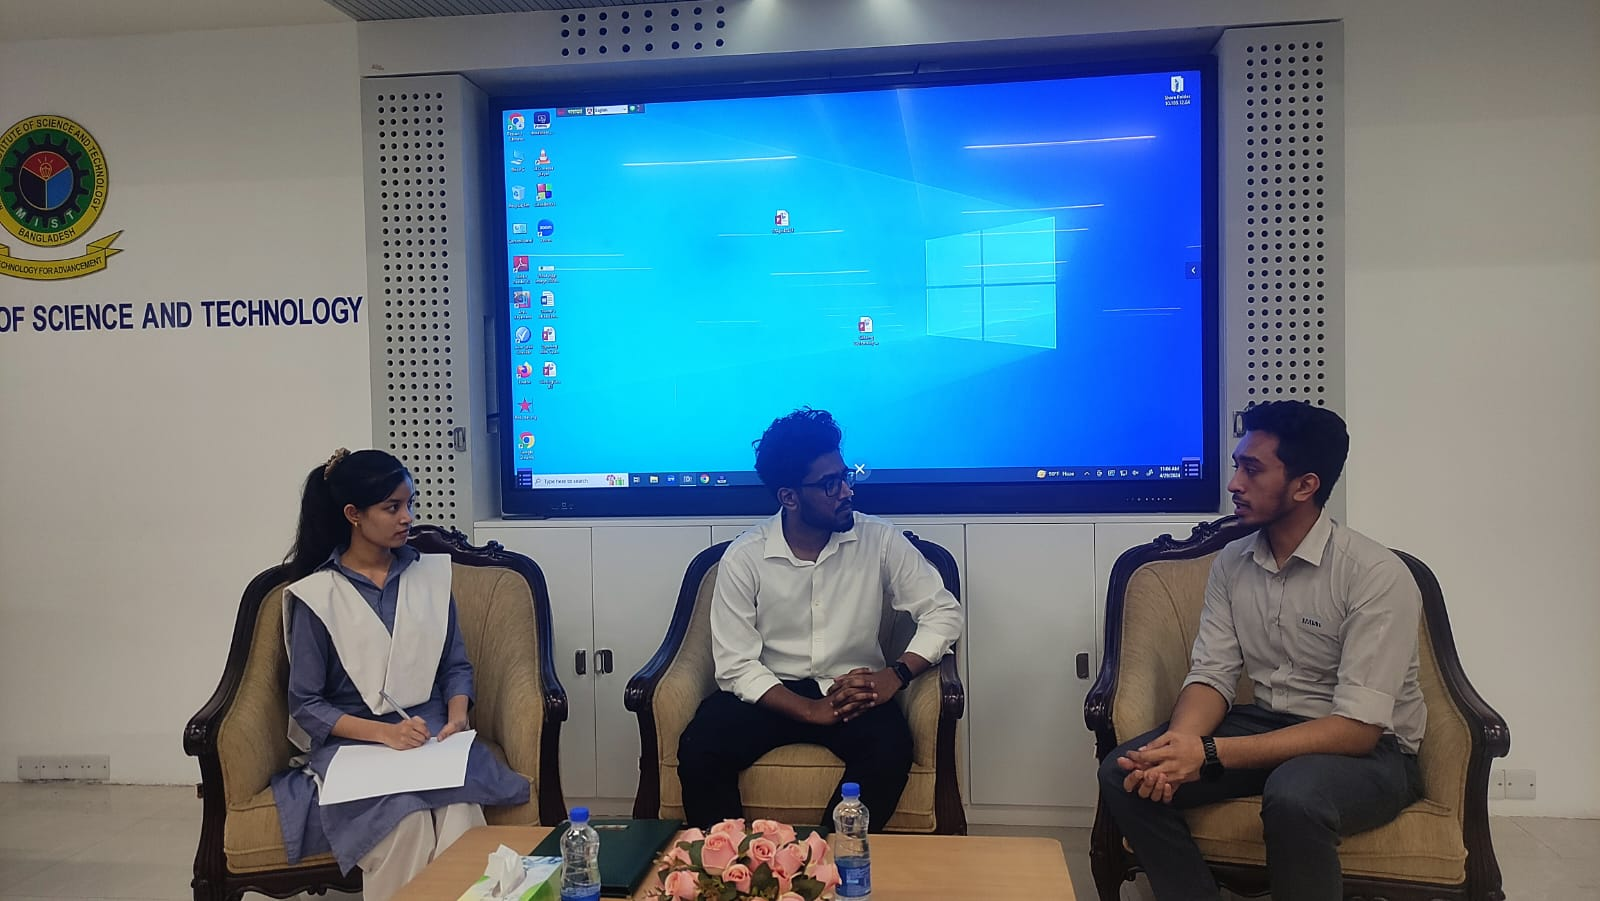
\includegraphics[width=0.7\linewidth]{mcsc.jpg}
    \caption{Inside Cyber-range with the President of MCSC}
    \label{fig:enter-label}
\end{figure}
\newpage
\subsection*{ Questionnaires:\\}

\begin{enumerate}
    \item {As a leading club in MIST, does MCSC have a website/app of its own for cybersecurity training or for other purposes?\\}

        \textbf{President of MCSC:} Unfortunately no, currently the club does not have a website/app of it's own, but we had plans of developing it.. But as our panel members are busy in their tasks/projects we couldn't make it possible, so maybe someday.\\
    \item {We were planning on creating a cybersecurity platform/website for students, participants, teachers, which might integrate with MCSC, if things go right. What do you think about it?\\}

        \textbf{President of MCSC:} That'd be a great initiative. As we talked earlier, being one of the best cyber clubs, MCSC doesn't have a Cybersecurity platform of it's own, which is a shame actually. Your initiative will be largely helpful for the club and the community.\\

    \item {What are the problems you faced while hosting CTF contests?\\}

        \textbf{President of MCSC:} For hosting any CTF contest, we have to rely on paid platforms. As of current date, we host our contests on RICSEC's platform but we had to pay a hefty sum for every question..\\
    
    \item {How do you share or organize all learning materials/resources of any certification course/class?\\}
    
        \textbf{President of MCSC:} We just give the materials to our fellow club members/students via our Messenger group or Discord server, but organizing them is upto students. So there are no organizing facilities to give students a structured cybersecurity learning path or roadmap.\\
\end{enumerate}  
\newpage
\subsection*{Survey of MCSC members\\}
\textbf{We surveyed the students and panel members of MCSC through Google Forms. A total of 14 people responded to our queries. Here are the results from the survey:\\}

\begin{figure}[H]
    \centering
    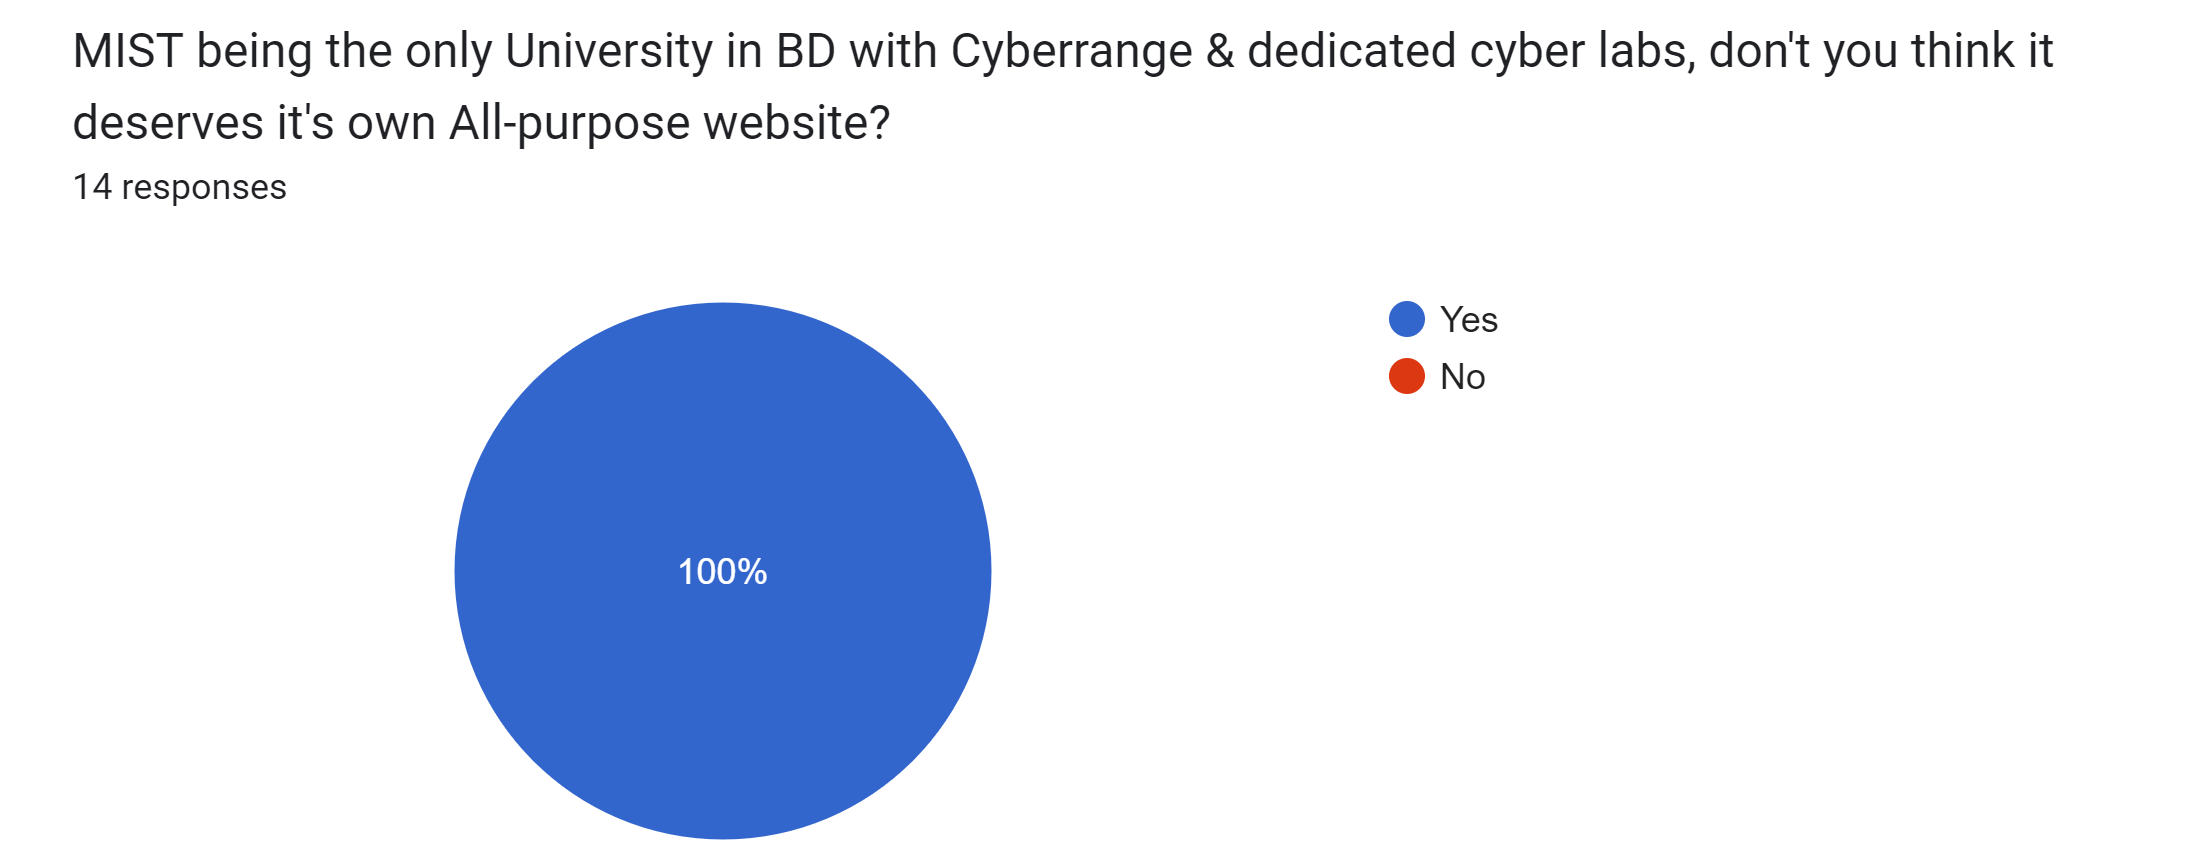
\includegraphics[width=1.0\linewidth]{Report/Picture1.png}
    \label{fig:picture1}
\end{figure}
\begin{figure}[H]
    \centering
    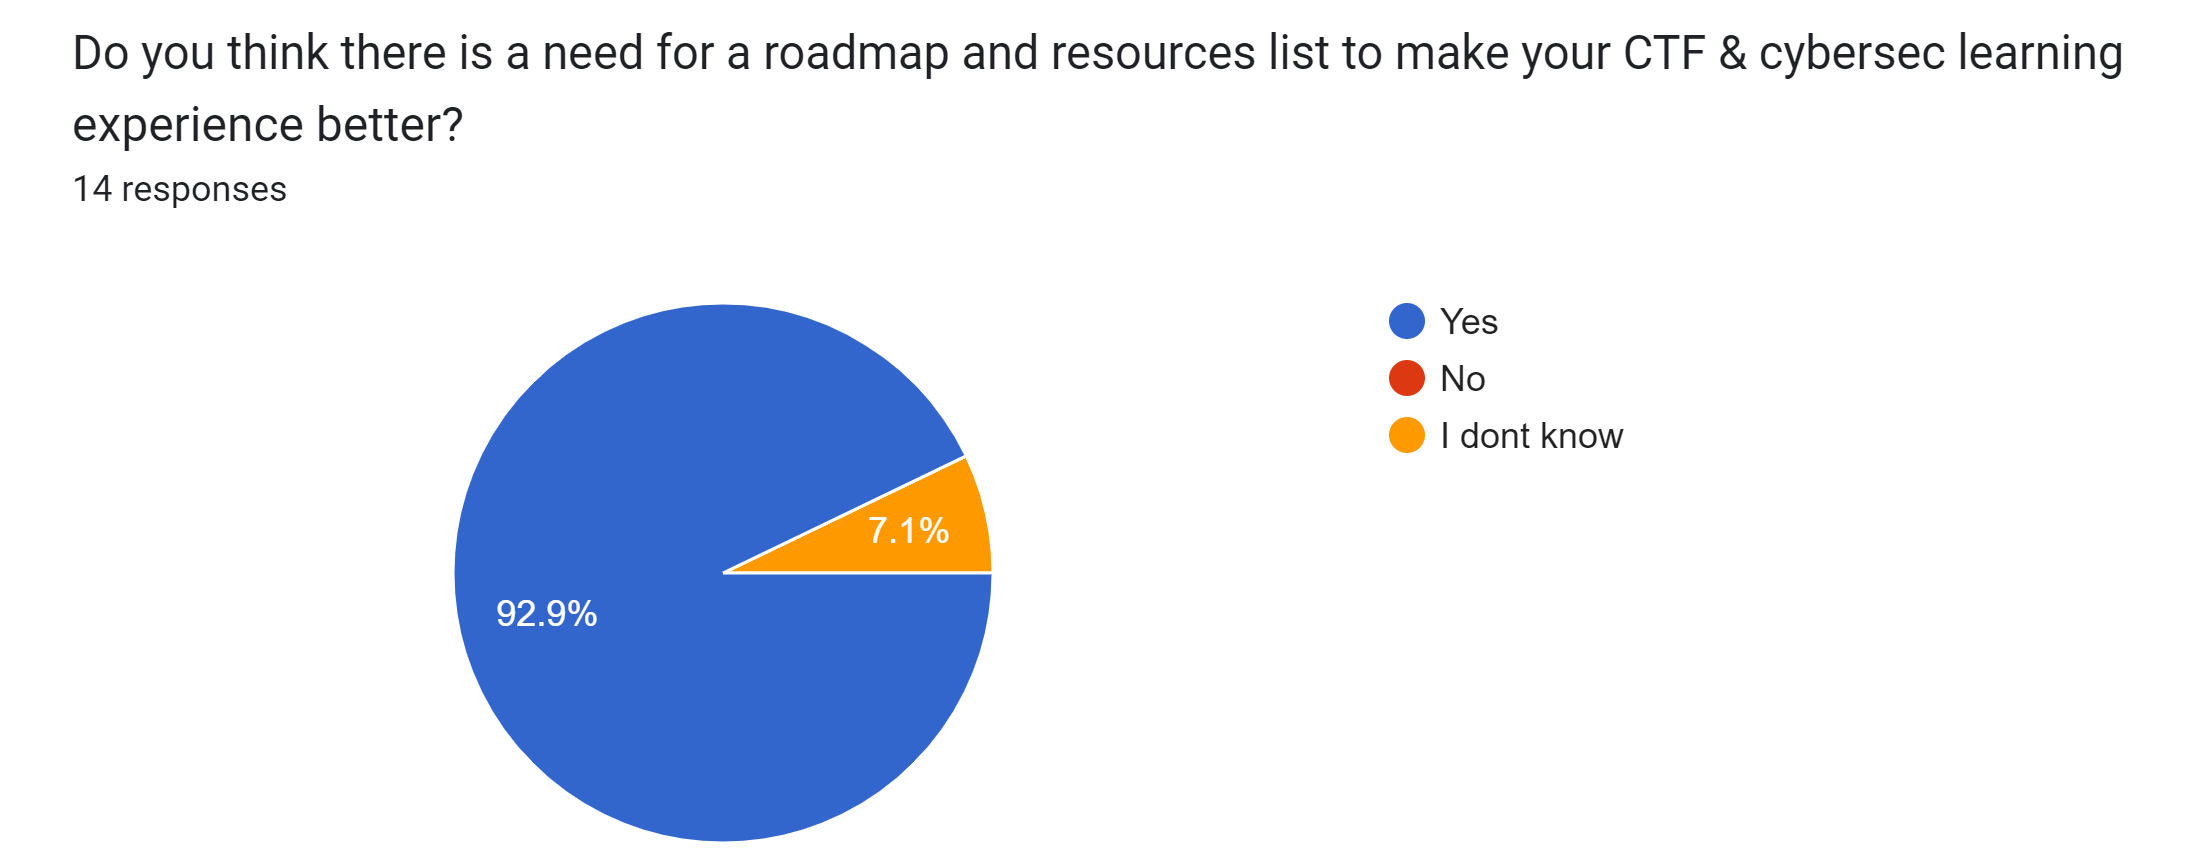
\includegraphics[width=1.0\linewidth]{Report/Picture3.png}
    \label{fig:picture3}
    
%\clearpage
\end{figure}
\begin{figure}[H]
    \centering
    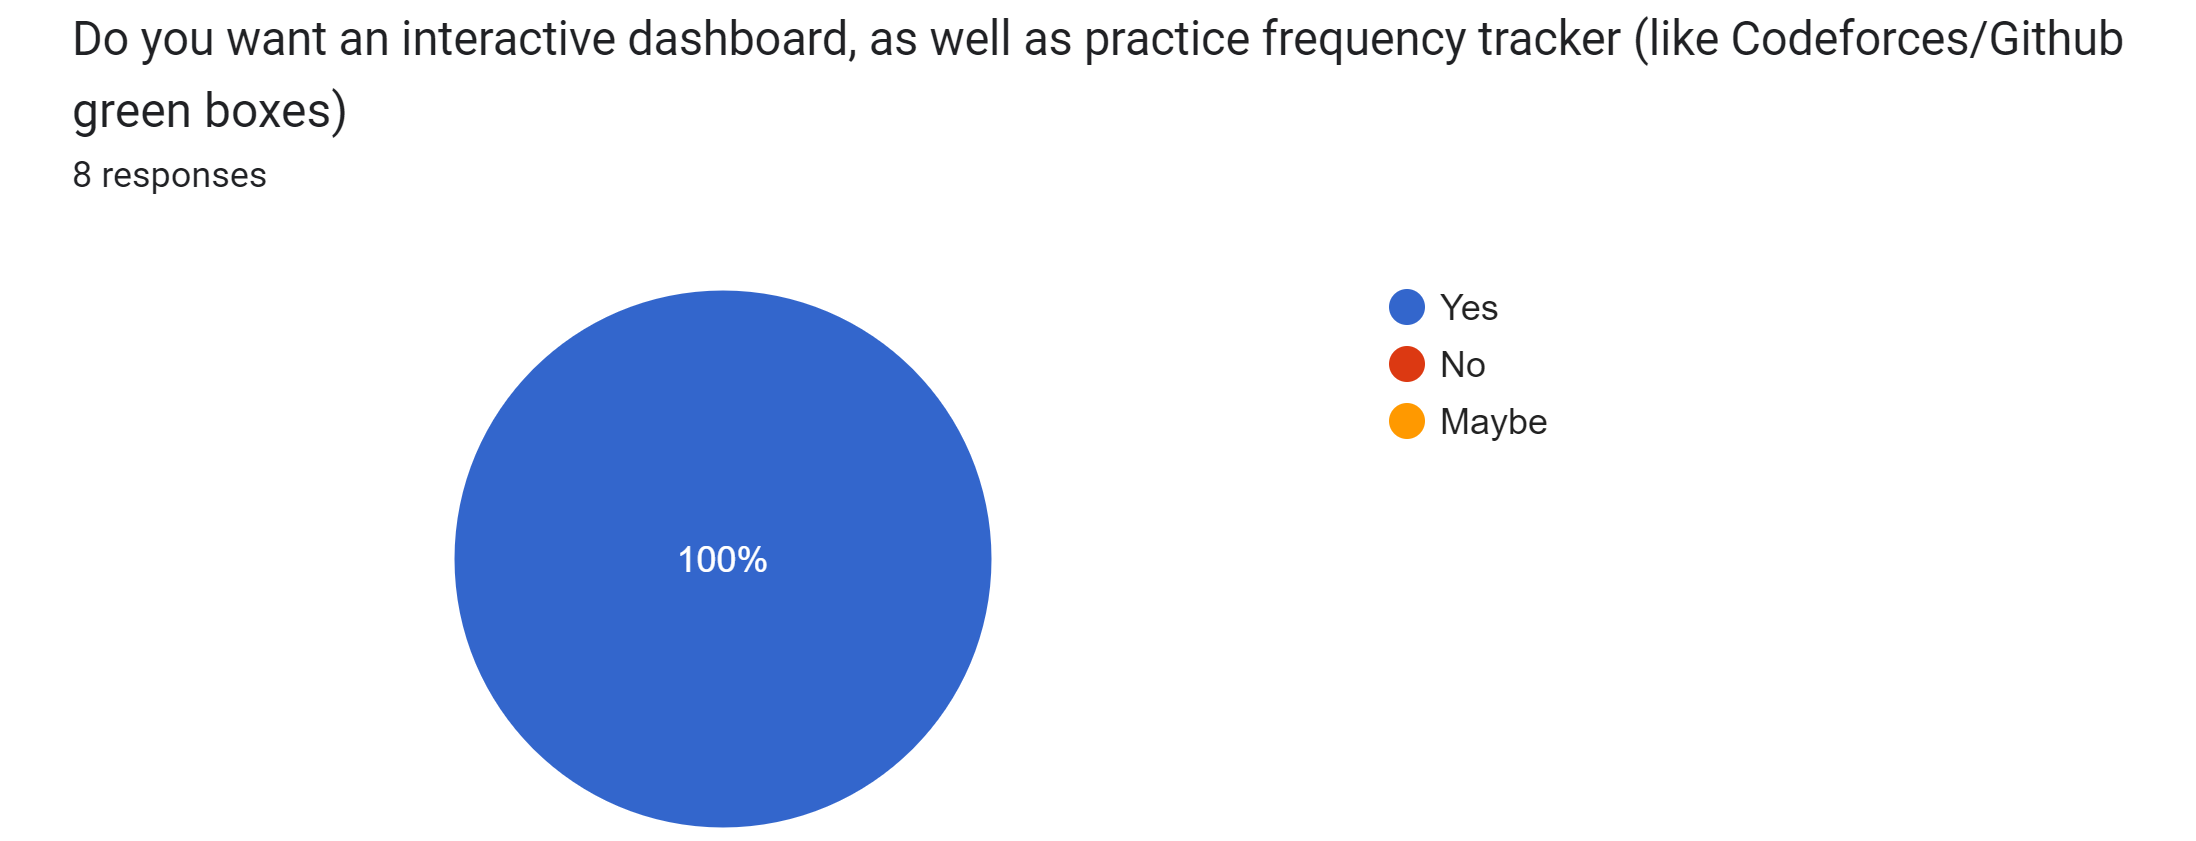
\includegraphics[width=1.0\linewidth]{Report/Picture5.png}
    \label{fig:picture5}
\end{figure}
\begin{figure}[H]
    \centering
    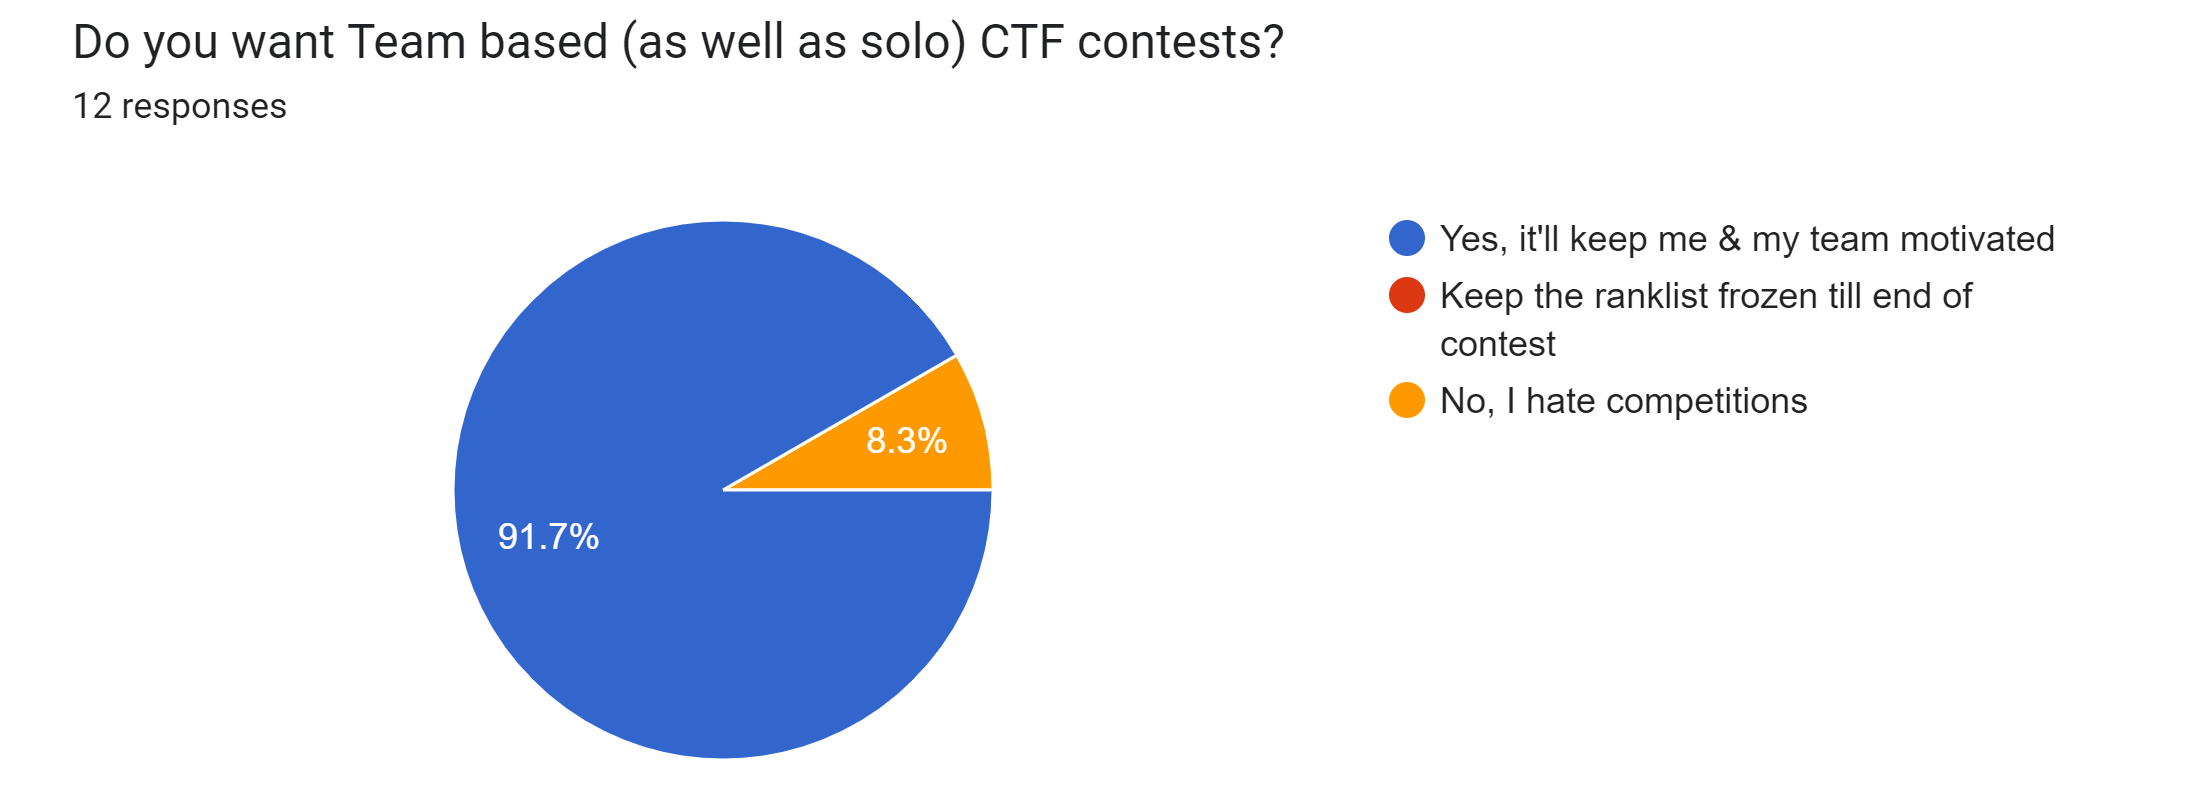
\includegraphics[width=1.0\linewidth]{Report/Picture6.png}
    \label{fig:picture6}
\end{figure}

\subsection*{Findings from the interview and survey:\\}
The interview with the President of the MIST Cyber Security Club (MCSC) and the survey reveals that the club currently lacks a dedicated website or app for cybersecurity training due to the busy schedules of its members. The President is highly supportive of the idea to create such a platform, seeing it as a beneficial initiative for the club and the community. MCSC faces financial challenges in hosting Capture the Flag (CTF) contests, as they have to pay significant fees to use platforms like RICSEC. Additionally, learning materials are shared informally through Messenger and Discord, with no structured system for organizing them, leaving students to manage thigns on their own.

% \section{Visiting organization: Brainstation-23}

% {Brainstation-23 is a software development company based in Bangladesh. It was founded in 2006 by Raisul Kabir. The company makes software for leading technological, fintech, banking  & many other industries in Bangladesh and abroad.

% We’ve talked with Raisul Kabir, the CEO and founder of Brainstation-23. As a large software company providing software for big name companies, they’ve to ensure the security of their applications and follow cybersecurity rules (like the ones defined by OWASP).\\}

% \subsection*{Questionnaires}:
% {

% }
\section*{Literature Review, Limitations and Proposed solution}

\subsection*{Title: Managing Escalating Cyber Threats: Perspectives and Policy Insights for Bangladesh}
\textbf{Source:} (Sayduzzaman et al., 2024) Sayduzzaman, M., Sazzad, S., Rahman, M., Rahman, T., \& Uddin, M. (2024). Managing Escalating Cyber Threats: Perspectives and Policy Insights for Bangladesh.\\
\textbf{Limitations:} There is a shortage of skilled cybersecurity professionals and technical equipment needed for effective cyberspace protection.\\
\textbf{Proposed solution:} To prevent cyberattacks, organizations need to train cybersecurity professionals, identify a cybersecurity partner and embrace a culture of security.

\subsection*{Title: Cyber Security Awareness in Bangladesh: An Overview of Challenges and Strategies}
\textbf{Source:} Mamun, A. A., Ibrahim, J. B., \& Mostofa, S. M. (2021). Cyber Security Awareness in Bangladesh: An Overview of Challenges and Strategies. 9(1).\\
\textbf{Limitations:} The associated organizations, as well as the government, are not concerned about cybercrime issues.\\
\textbf{Proposed solution:} Bangladesh needs a specific strategic approach and specific doctrines to fulfill the requirement of cyber-security. If people had previous knowledge of cyber security weaknesses, they would end up finding ways to defend themselves.

\subsection*{Title: Need for Cyber Defense, Security Strategy and Privacy Policy in Bangladesh - Hype or Reality?}
\textbf{Source:} Bahalul Haque, A. (2019). NEED FOR CRITICAL CYBER DEFENCE, SECURITY STRATEGY AND PRIVACY POLICY IN BANGLADESH - HYPE OR REALITY? International Journal of Managing Information Technology, 11(01), 37–50. https://doi.org/10.5121/ijmit.2019.11103\\
\textbf{Limitations:} People still are not aware of their data being taken away or data theft. There is no explicit data privacy and protection law in Bangladesh.\\
\textbf{Proposed solution:} We should have a continuous evaluation of cyber security events. This can be achieved through association with private-public organizations both nationally and globally.

\subsection*{Title: Cyber Crime Trend in Bangladesh, an Analysis and Ways Out to Combat the Threat}
\textbf{Source:} (Kundu et al., 2018) Kundu, S., Islam, K., Jui, T., Rail, S., Hossain, D., \& Chowdhury, I. (2018). Cyber crime trend in Bangladesh, an analysis and ways out to combat the threat. 474–480. https://doi.org/10.23919/ICACT.2018.8323800\\
\textbf{Limitations:} The current cyber attack trend in Bangladesh demands attention for creating and maintaining a robust and workable cyber security strategy.\\
\textbf{Proposed solution:} Various seminars and workshops should be arranged to create public awareness.
\newpage
\section*{Users and Their Roles}
\begin{enumerate}
    \item \textbf{Organizers:}
        \begin{enumerate}
            \item Can organize contests free of cost.
            \item See standings.
            \item Can see upcoming programs.
        \end{enumerate}
    \item \textbf{Contestants:}
        \begin{enumerate}
            \item Participate in contests.
            \item Standings.
            \item Ratings.
            \item Easy access to learning materials.
            \item Keep track of practice activity.
            \item Can see upcoming programs.
        \end{enumerate}
    \item \textbf{Educators:}
        \begin{enumerate}
            \item Learning materials.
            \item Contribution.
            \item Can see the performance of students.
            \item Can see upcoming programs.
        \end{enumerate}
    \item \textbf{Students:}
        \begin{enumerate}
            \item Enroll in courses.
            \item Submit assignments.
        \end{enumerate}
\end{enumerate}
% \newpage
\section*{Features:}
\begin{enumerate}
    \item \textbf{Authentication:} User management, Secured user auth.
    \item \textbf{CTF Management:} Store CTF categories and CTFs according to their category.
    \item \textbf{CTF Contest Type:} Team or solo CTF participation.
    \item \textbf{Learning Path and Resources:} Stores them in separate tables.
    \item \textbf{Course Enrollment \& Management:} User can enroll in courses free of cost.
    \item \textbf{Dashboard and Scoreboard:} Interactive dashboard and real-time updating scoreboard.
    \item \textbf{Activity Heatmap:} Keeps record of daily streak.
\end{enumerate}
\newpage

\section*{Possible  Tables}

\begin{itemize}
    \item \textbf{User}
    \begin{itemize}
        \item User\_id
        \item Username
        \item Password
        \item Email
        \item Oauth\_id
        \item Team id
        \item Verified
        \item Country
        \item Banned
        \item Hidden
    \end{itemize}

    \item \textbf{Host}
    \begin{itemize}
        \item Rating
        \item Cur\_Contests
        \item Tokens
        \item Prev\_contest
    \end{itemize}
    
    \item \textbf{Challenges}
    \begin{itemize}
        \item Challenge\_id
        \item Name
        \item Description
        \item Flag
        \item Max attempt
        \item Point
        \item Category
        \item Hint
        \item Hint\_cost
        \item Hint\_active
    \end{itemize}

    \item \textbf{Team}
    \begin{itemize}
        \item Team id
        \item Team name
        \item Member\_ids
    \end{itemize}
    
    \item \textbf{Contest}
    \begin{itemize}
        \item Contest\_id
        \item Start\_time
        \item End\_time
        \item Description
        \item Contest\_name
    \end{itemize}

    \item \textbf{Submission}
    \begin{itemize}
        \item Submission\_id
        \item User\_id
        \item Team\_id
        \item Count
        \item Time
        \item Is\_Correct
        \item Penalty
        \item Points
    \end{itemize}

    \item \textbf{Instructor}
    \begin{itemize}
        \item Instr\_Id
        \item Course\_Tokens
        \item Specializations
        \item Education
        \item Affiliations
        \item Website
        \item Penalty
    \end{itemize}

    \item \textbf{Course}
    \begin{itemize}
        \item Course\_id
        \item Course\_Name
        \item Instructors
        \item Students
        \item Instr\_Token
        \item Student\_Token
        \item Fees
    \end{itemize}
\newpage
    \item \textbf{Lecture}
    \begin{itemize}
        \item Lecture\_Id
        \item Lecturer
        \item Link
        \item Date\_Posted
        \item C\_id
    \end{itemize}

    \item \textbf{Materials}
    \begin{itemize}
        \item Material\_id
        \item C\_id
        \item Type
        \item Content
    \end{itemize}

    \item \textbf{Assignments}
    \begin{itemize}
        \item Assgn\_id
        \item C\_id
        \item instr\_id
        \item Description
        \item Deadline
        \item Marks
        \item Submitted\_by
        \item Submissions
        \item Marks\_obtained
        \item Date\_Submitted
    \end{itemize}
\end{itemize}





% ----------------------------------------------------------------------
% Conclusion
% ----------------------------------------------------------------------


\end{document}